\section{Specific Requirements}

\subsection{External Interfaces}

\subsubsection{System Interfaces}

\paragraph{Municipality Data Exchange} \label{p:mde} The definition of the municipality data exchange interface is dependent to the corresponding SafeStreet's interface required to be offered to the municipalities. The municipality is required to offer the following functionalities to the system:

	\begin{itemize}
		\item Guarantee a secure authentication to the municipalities' system using a provided \emph{restricted access API}
		\item Provide a secure transfer of data related to accidents occurred in the territory of the municipality
		\item Provide a secure transfer of data related to local authorities' issued tickets 
	\end{itemize} 
	
	Leveraging the retrieved municipality data the system is required to cross this information with the system previously stored data. In addition, the system is required to perform the following functions on the crossed data:
	
	\begin{itemize}
		\item Build statistics on the frequency of violations
		\item Build statistics on the users that submit the most violations
		\item Build statistics on the cities with the highest number of violations
		\item Build statistics on the effectiveness of the SafeStreets initiative by looking for trends in the issuing of tickets
		\item Identify potentially unsafe areas and store this new generated information 
		\item Identify possible interventions to be suggested to the municipalities and store this new generated information 
	\end{itemize}
		
	To fulfil the bidirectional data exchange the system is required to offer the following functionalities to the municipalities:
	
	\begin{itemize}
		\item Guarantee a secure authentication to the system using a provided \emph{restricted access API}
		\item Provide a secure transfer of data related to user uploaded violations and all the corresponding metadata
		\item Provide a secure transfer of data related to possible interventions suggestions 
		
	\end{itemize} 
	
\clearpage

\paragraph{Geographic Information System} \label{p:gis} The definition of the external GIS interface is GIS dependant and will be described in a functionality-based way. The system is required to perform the following functions:

	\begin{itemize}
		\item Load and filter data based on the user requested criteria
		\item Cache retrieved data for the most common user requested criteria
		\item Communicate the loaded and filtered data to the external GIS with the final goal of presenting the requested map to the user via the user interfaces
		
		\end{itemize}
	
	The system via the external GIS is required to be capable of handling the following data visualisations:
	
	\begin{itemize}
		\item Visualise the spatial location of stored violations inside a specific geographic area requested by the user
		\item Visualise the spatial location of stored violations inside a specific geographic area and a specific time range requested by the user
		\item Visualise the distinction between possible safe and unsafe areas identified by the system
		\item Map quantities and concentrations, such as where the most and least number of violations occurred, highlighting the streets (and areas) with the highest frequency of violations
		\item Map the change of quantities and concentrations inside a specific geographic area and a specific time range requested by the user \newline
	\end{itemize}

	\begin{figure}[h]
		\centering
		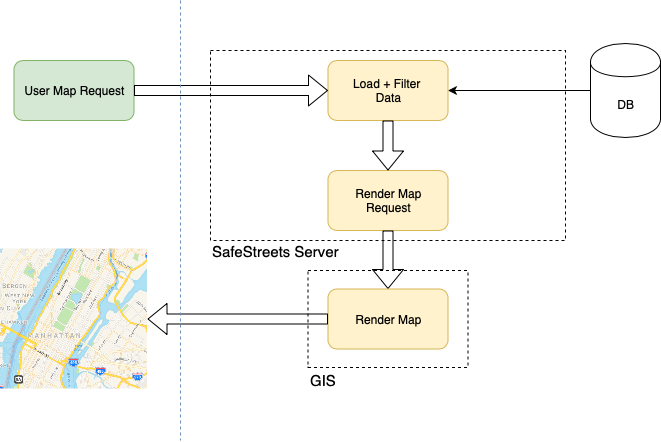
\includegraphics[width=335pt]{diagrams/GIS.png}
		\caption{
			\label{fig:externalGIS} GIS Interaction Diagram}
	\end{figure}

\subsubsection{User Interfaces}

	One of the key methodologies to capture the goals that the system's user interfaces must satisfy is through user interfaces mockups. The same structure of the overall description \hyperref[sec:goals]{corresponding section} will be used in order to extend the already stated requirements.

 \paragraph{Guest User}

	\begin{itemize}
		\item The system is required to offer guest users the ability to register to the system. The personal ID and a valid e-mail address are required for the registration in order to verify the authenticity of the new account. A password policy, composed of a set of rules designed to enhance security issues, is required to be forced to the user.
				
		\item The system is required to offer already registered guest users the ability to authenticate and log-in to the system. The system is required to offer the possibility to choose between a username, e-mail or personal ID log-in. \newline\newline
			
			\begin{figure}[h]
  				\centering
  				\begin{minipage}[b]{0.4\textwidth}
    				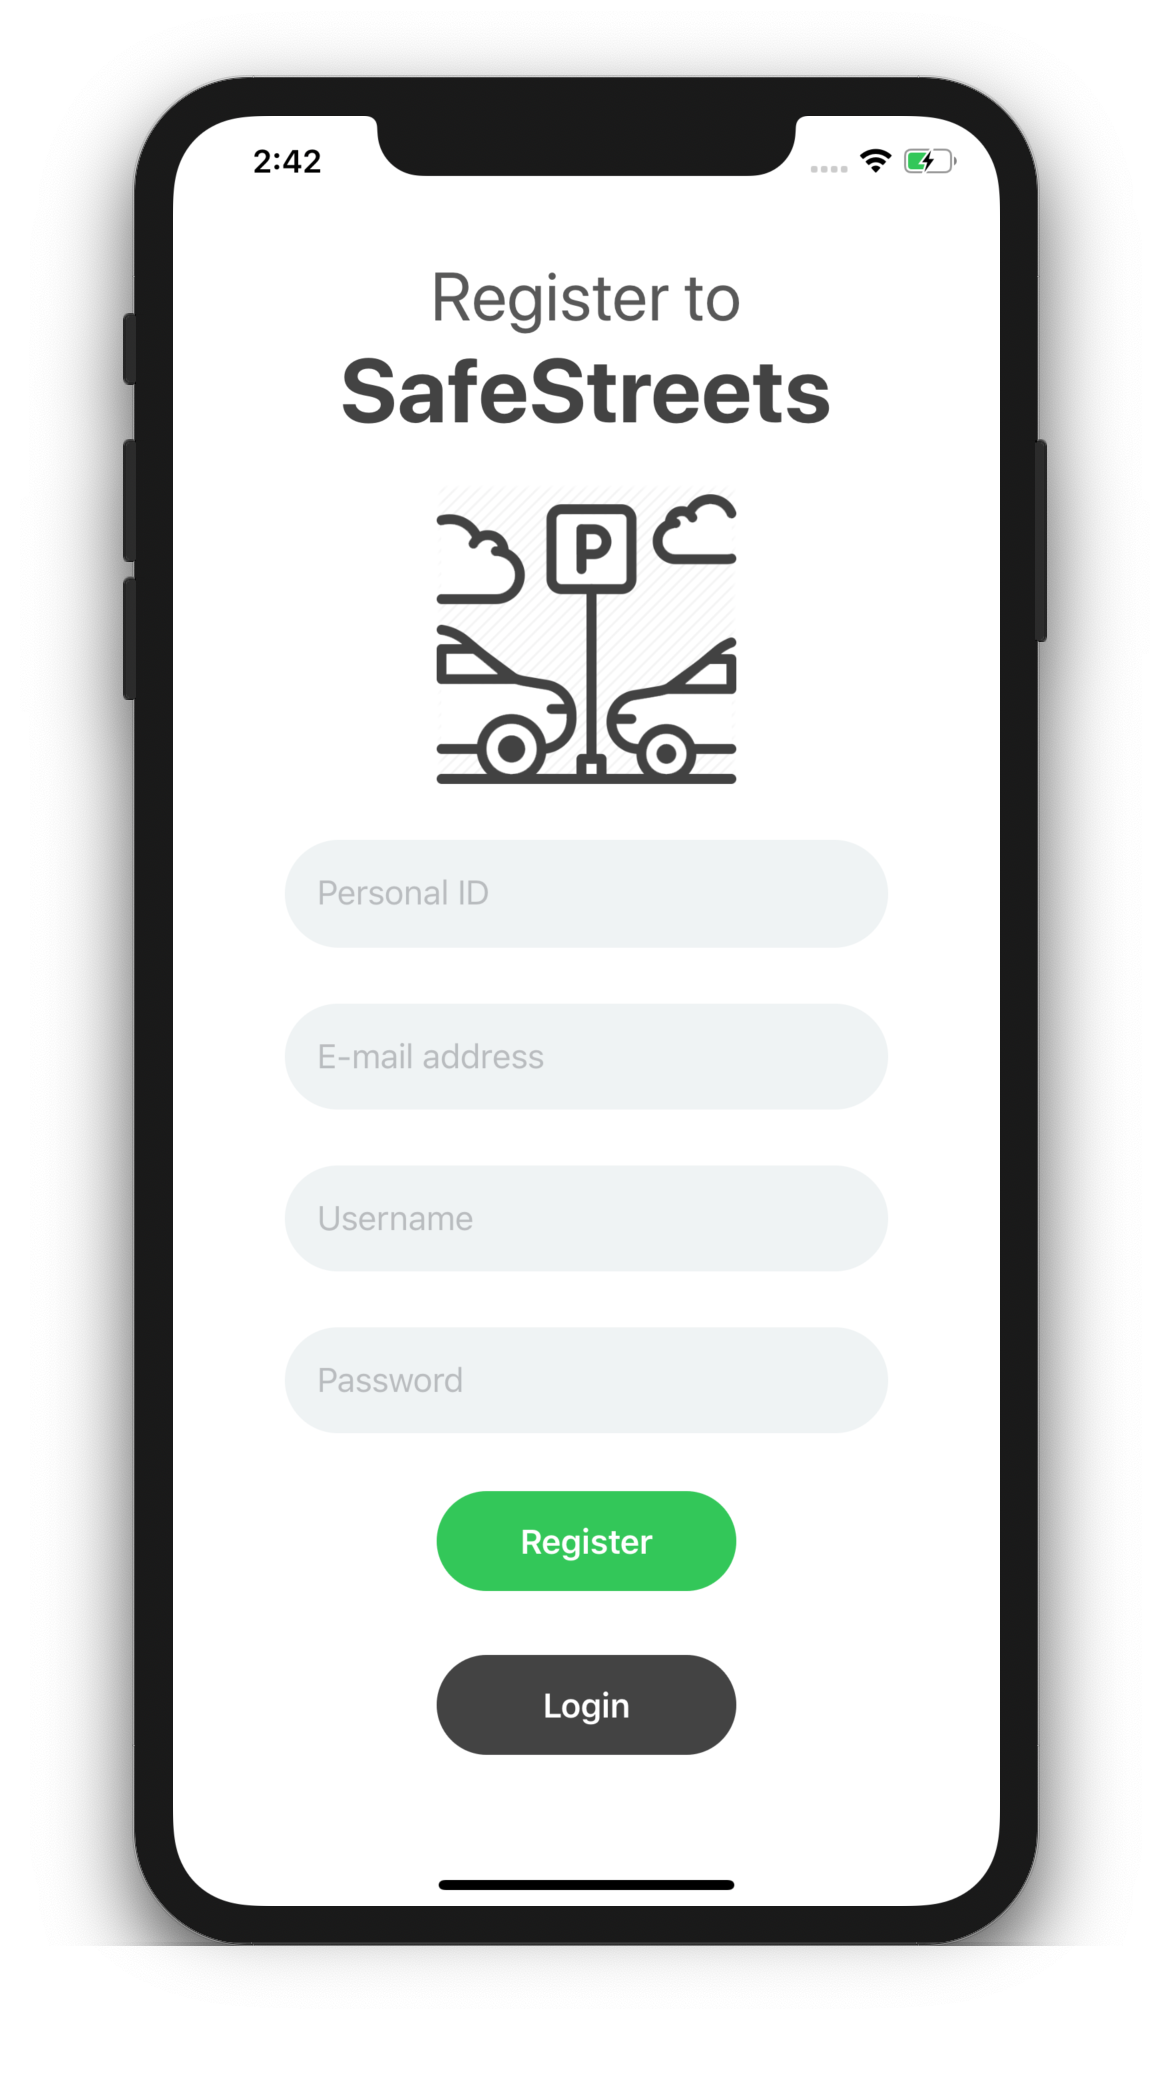
\includegraphics[width=\textwidth]{mockups/register-empty.png}
    					\caption{Registration Empty}
  				\end{minipage}
  				\hfill
  				\begin{minipage}[b]{0.4\textwidth}
    				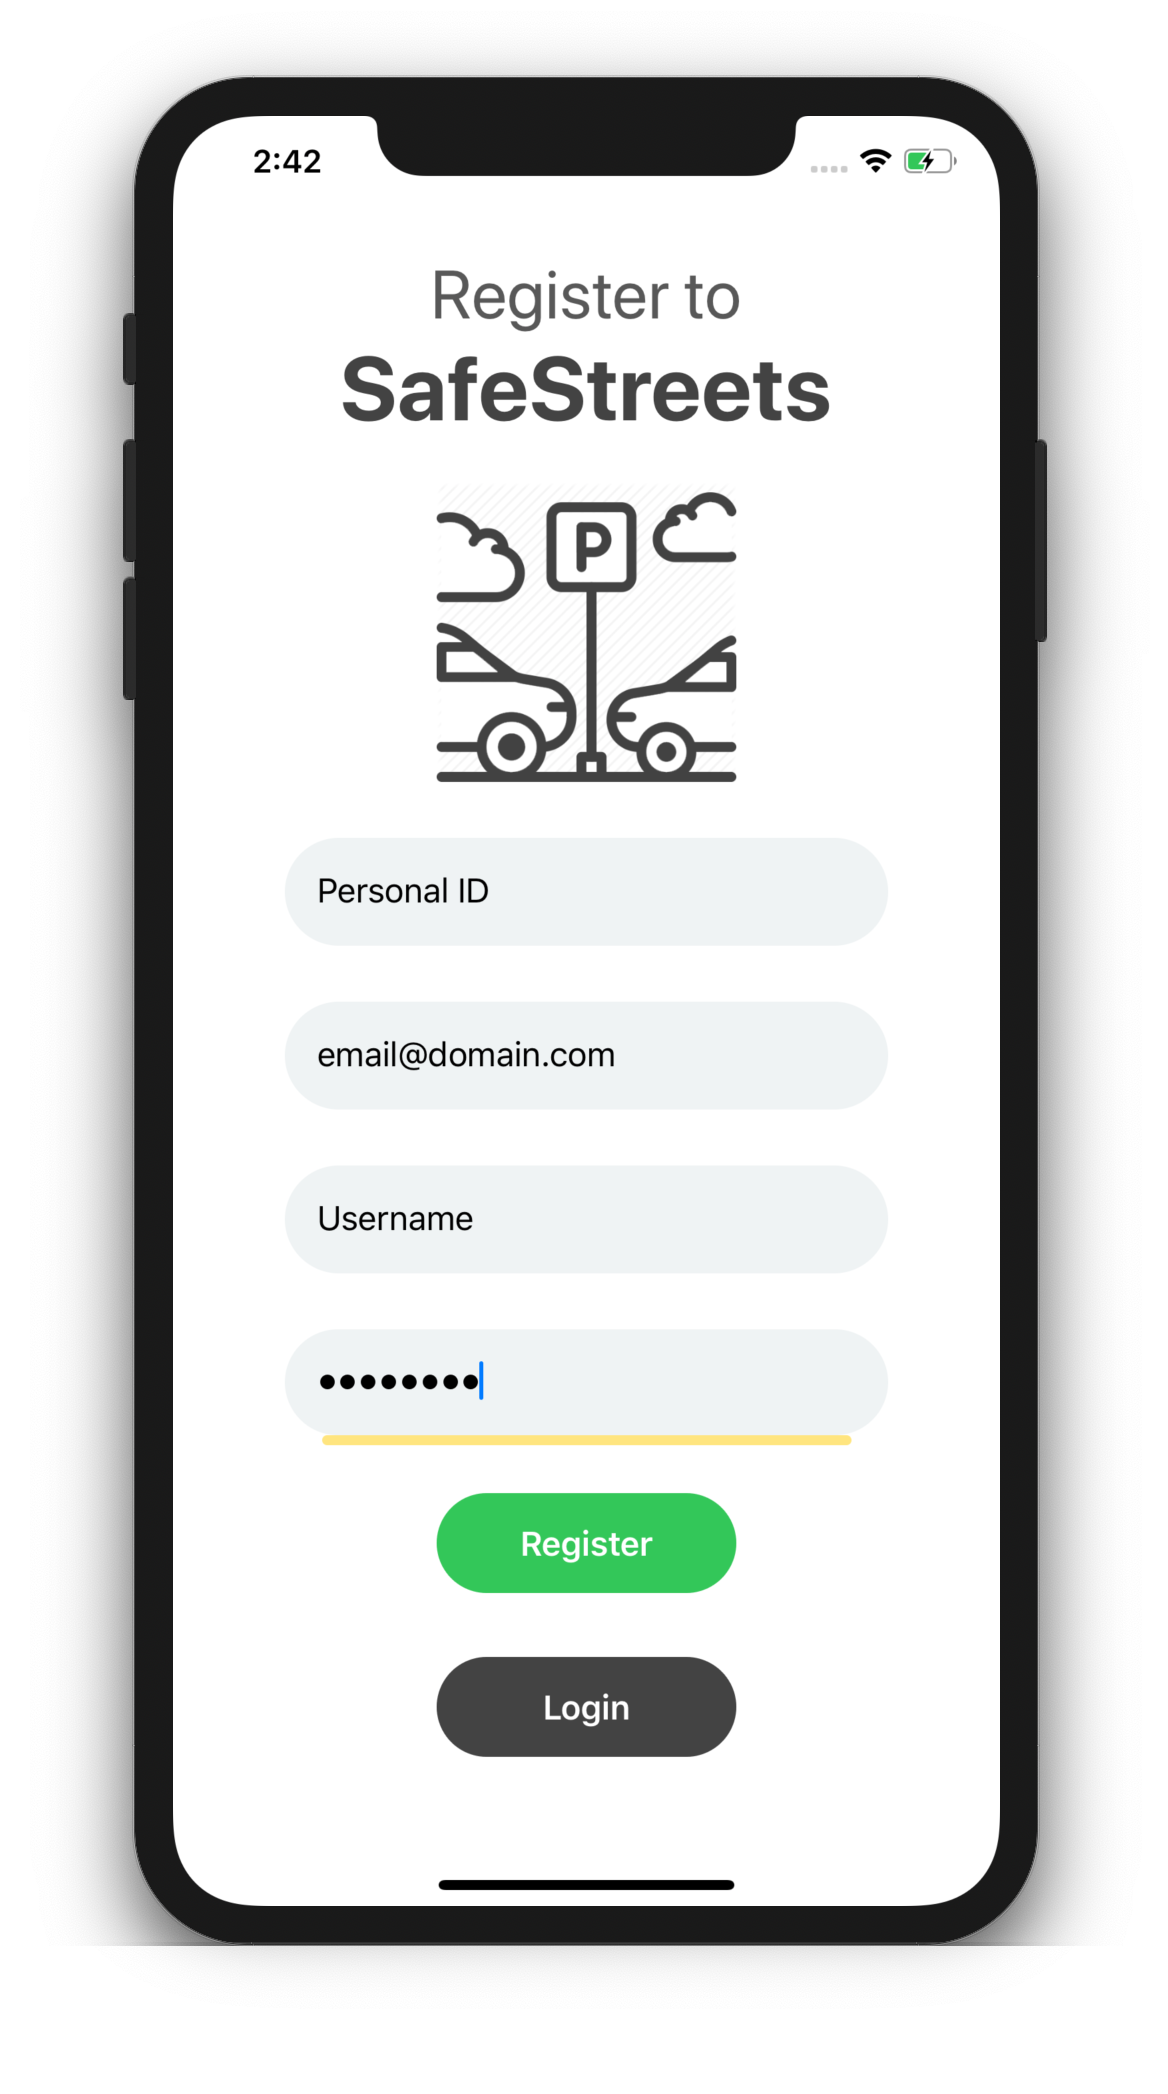
\includegraphics[width=\textwidth]{mockups/register.png}
    				\caption{Registration Filled}
  				\end{minipage}
			\end{figure}
		
			\begin{figure}[h]
  				\centering
  				\begin{minipage}[b]{0.4\textwidth}
    				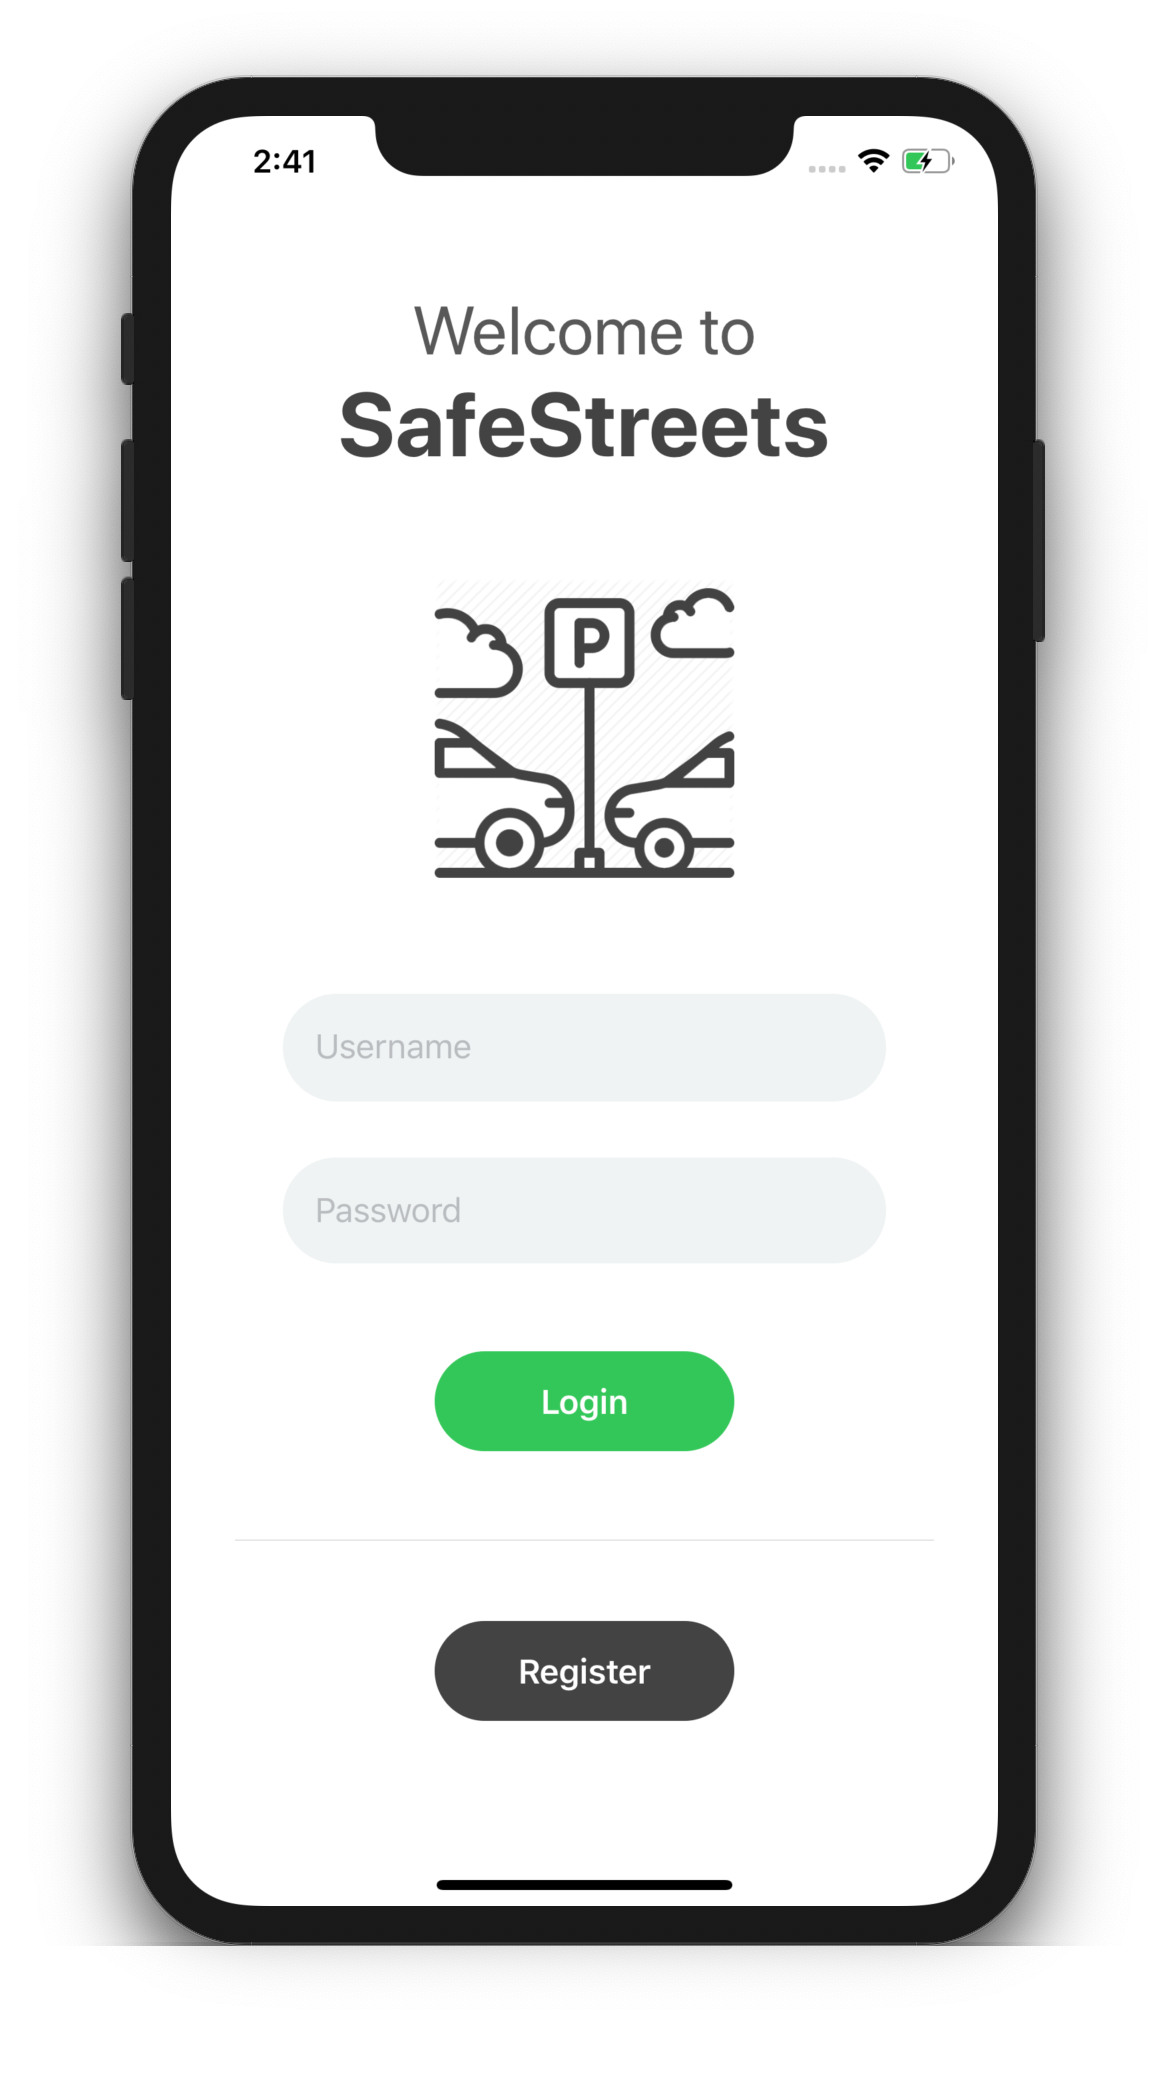
\includegraphics[width=\textwidth]{mockups/login-empty.png}
    					\caption{Login Empty}
  				\end{minipage}
  				\hfill
  				\begin{minipage}[b]{0.4\textwidth}
    				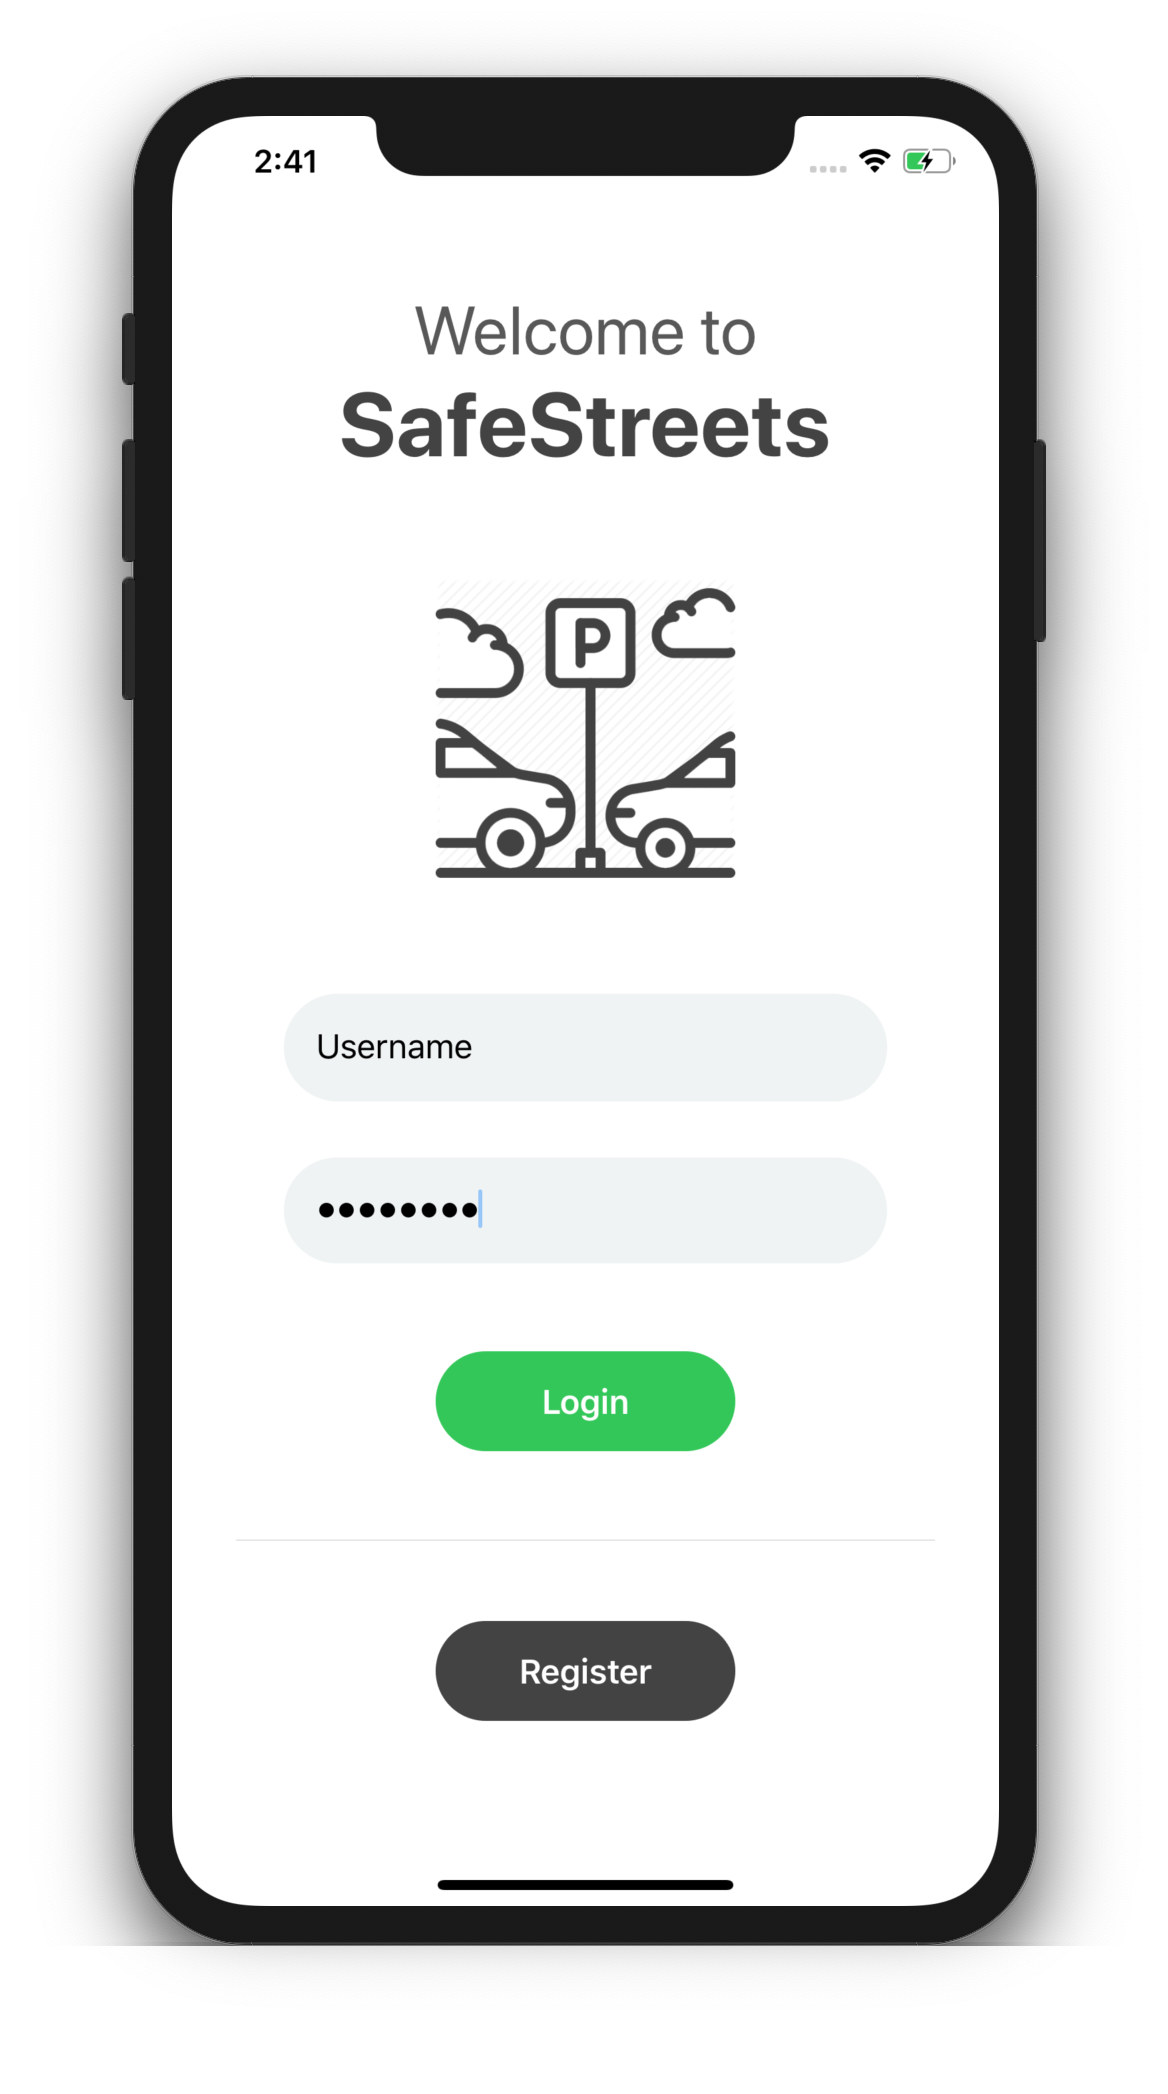
\includegraphics[width=\textwidth]{mockups/login.png}
    				\caption{Username Login}
  				\end{minipage}
			\end{figure}
			
	\end{itemize}



\newpage\paragraph{Logged User}
	\begin{itemize}
		\item The system is required to permit logged users to submit a violation. The submission is required to include a live photo captured via the \hyperref[sec:hardwareinterfaces]{hardware interfaces} of the user's device. The license plate number of the vehicle represented in the captured photo is not a mandatory field for the violation submission, but it will be leveraged for image recognition support if present. The user interface is required to allow the user to select the type of the committed violation from a predefined list of possible violations..			
		
		\item The system is required to allow logged users to consult a map through an external GIS and handle the different data visualisations discussed in the \hyperref[p:mde]{Municipality Data Exchange} section.
					 
			
			
		\item The system is required to allow logged users to consult the different statistics generated upon the system and the municipality collected data listed in the \hyperref[p:mde]{Geographic Information System} section.
		\item The system is required to allow logged users to view and edit the stored personal information in a profile section of the user interface and to log-out from the system. \newline\newline
			
			\begin{figure}[h]
  				\centering
  				\begin{minipage}[b]{0.4\textwidth}
    				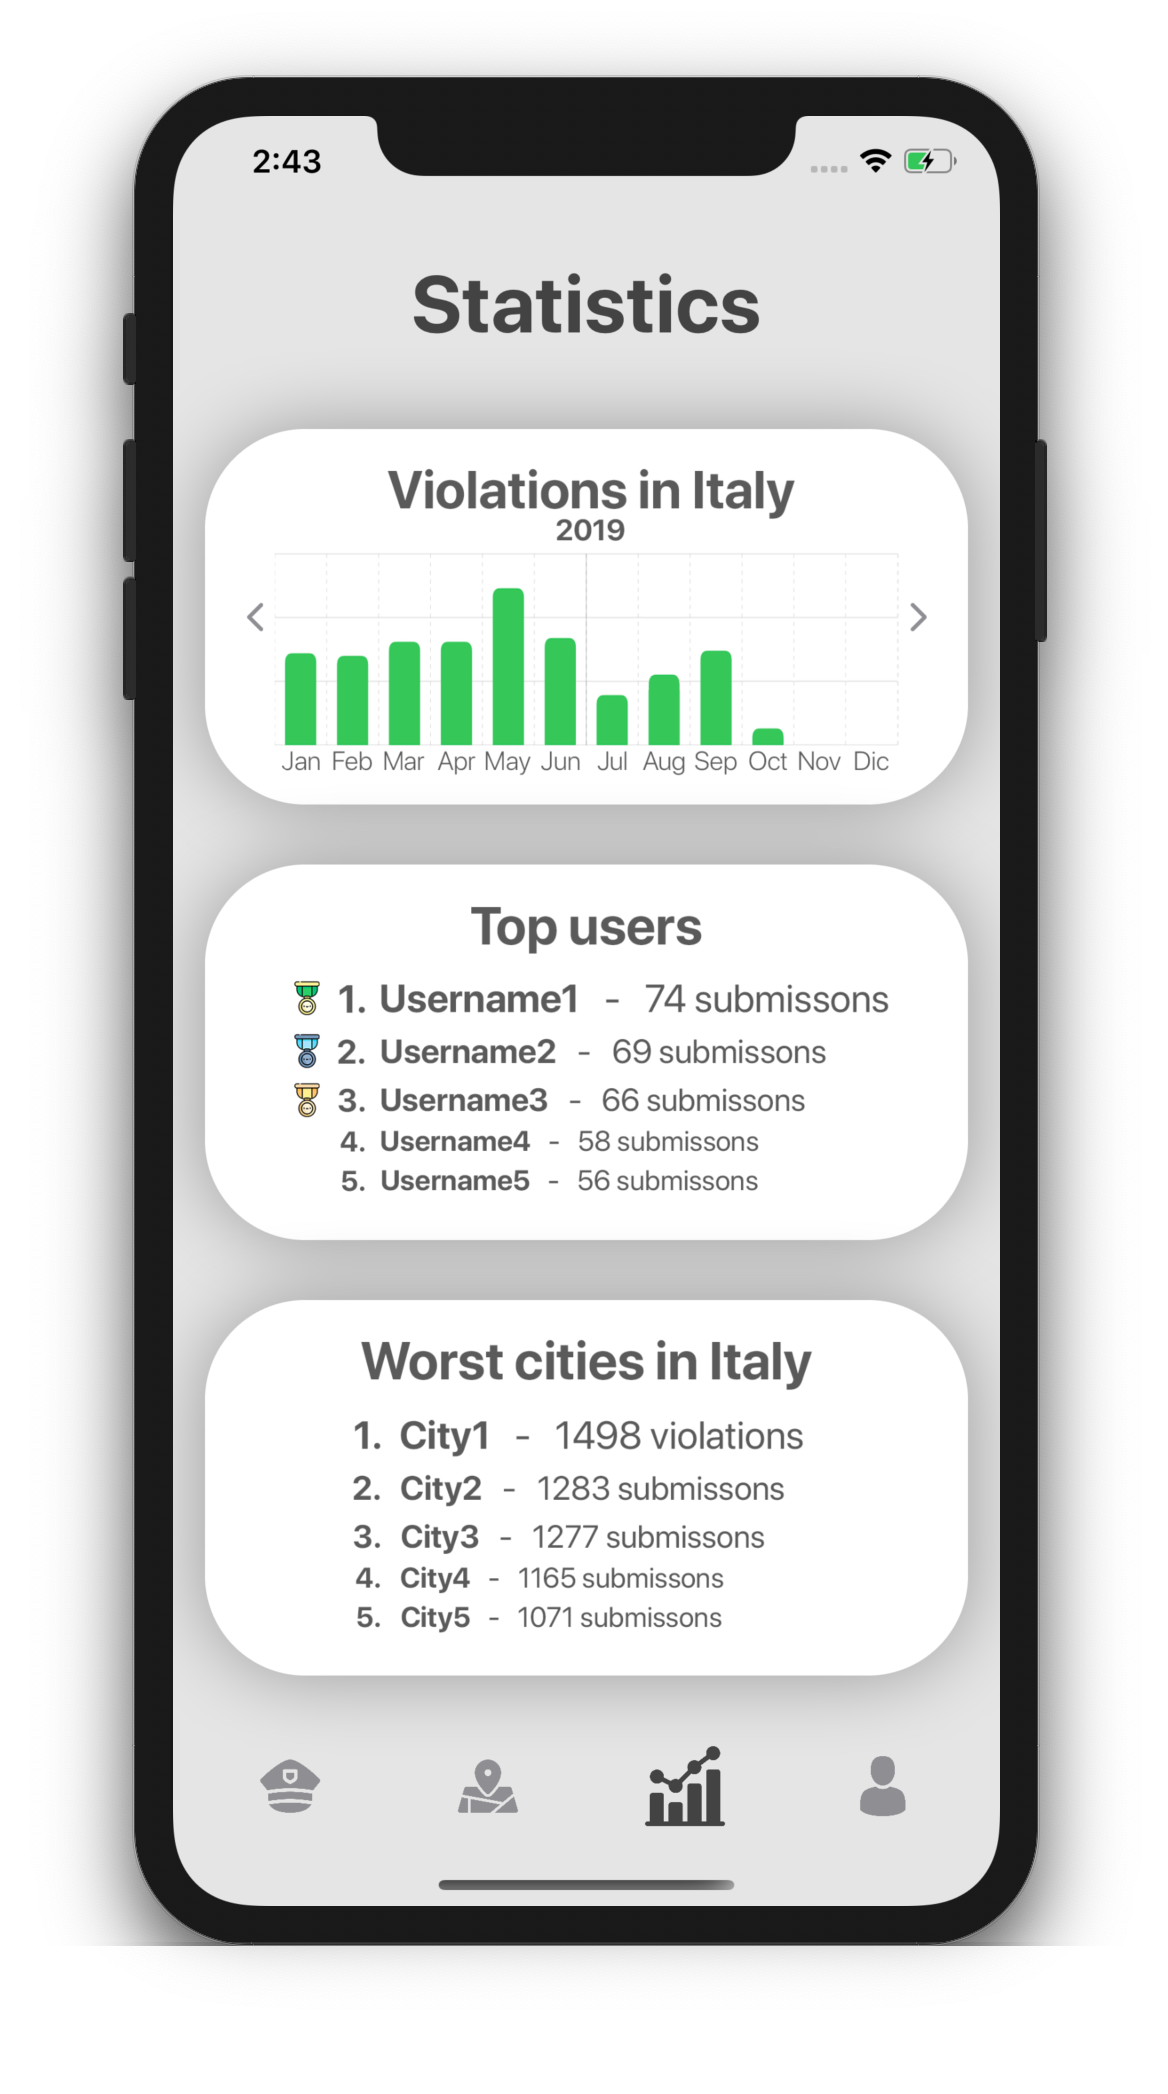
\includegraphics[width=\textwidth]{mockups/statistics.png}
    					\caption{Statistics View}
  				\end{minipage}
  				\hfill
  				\begin{minipage}[b]{0.4\textwidth}
    				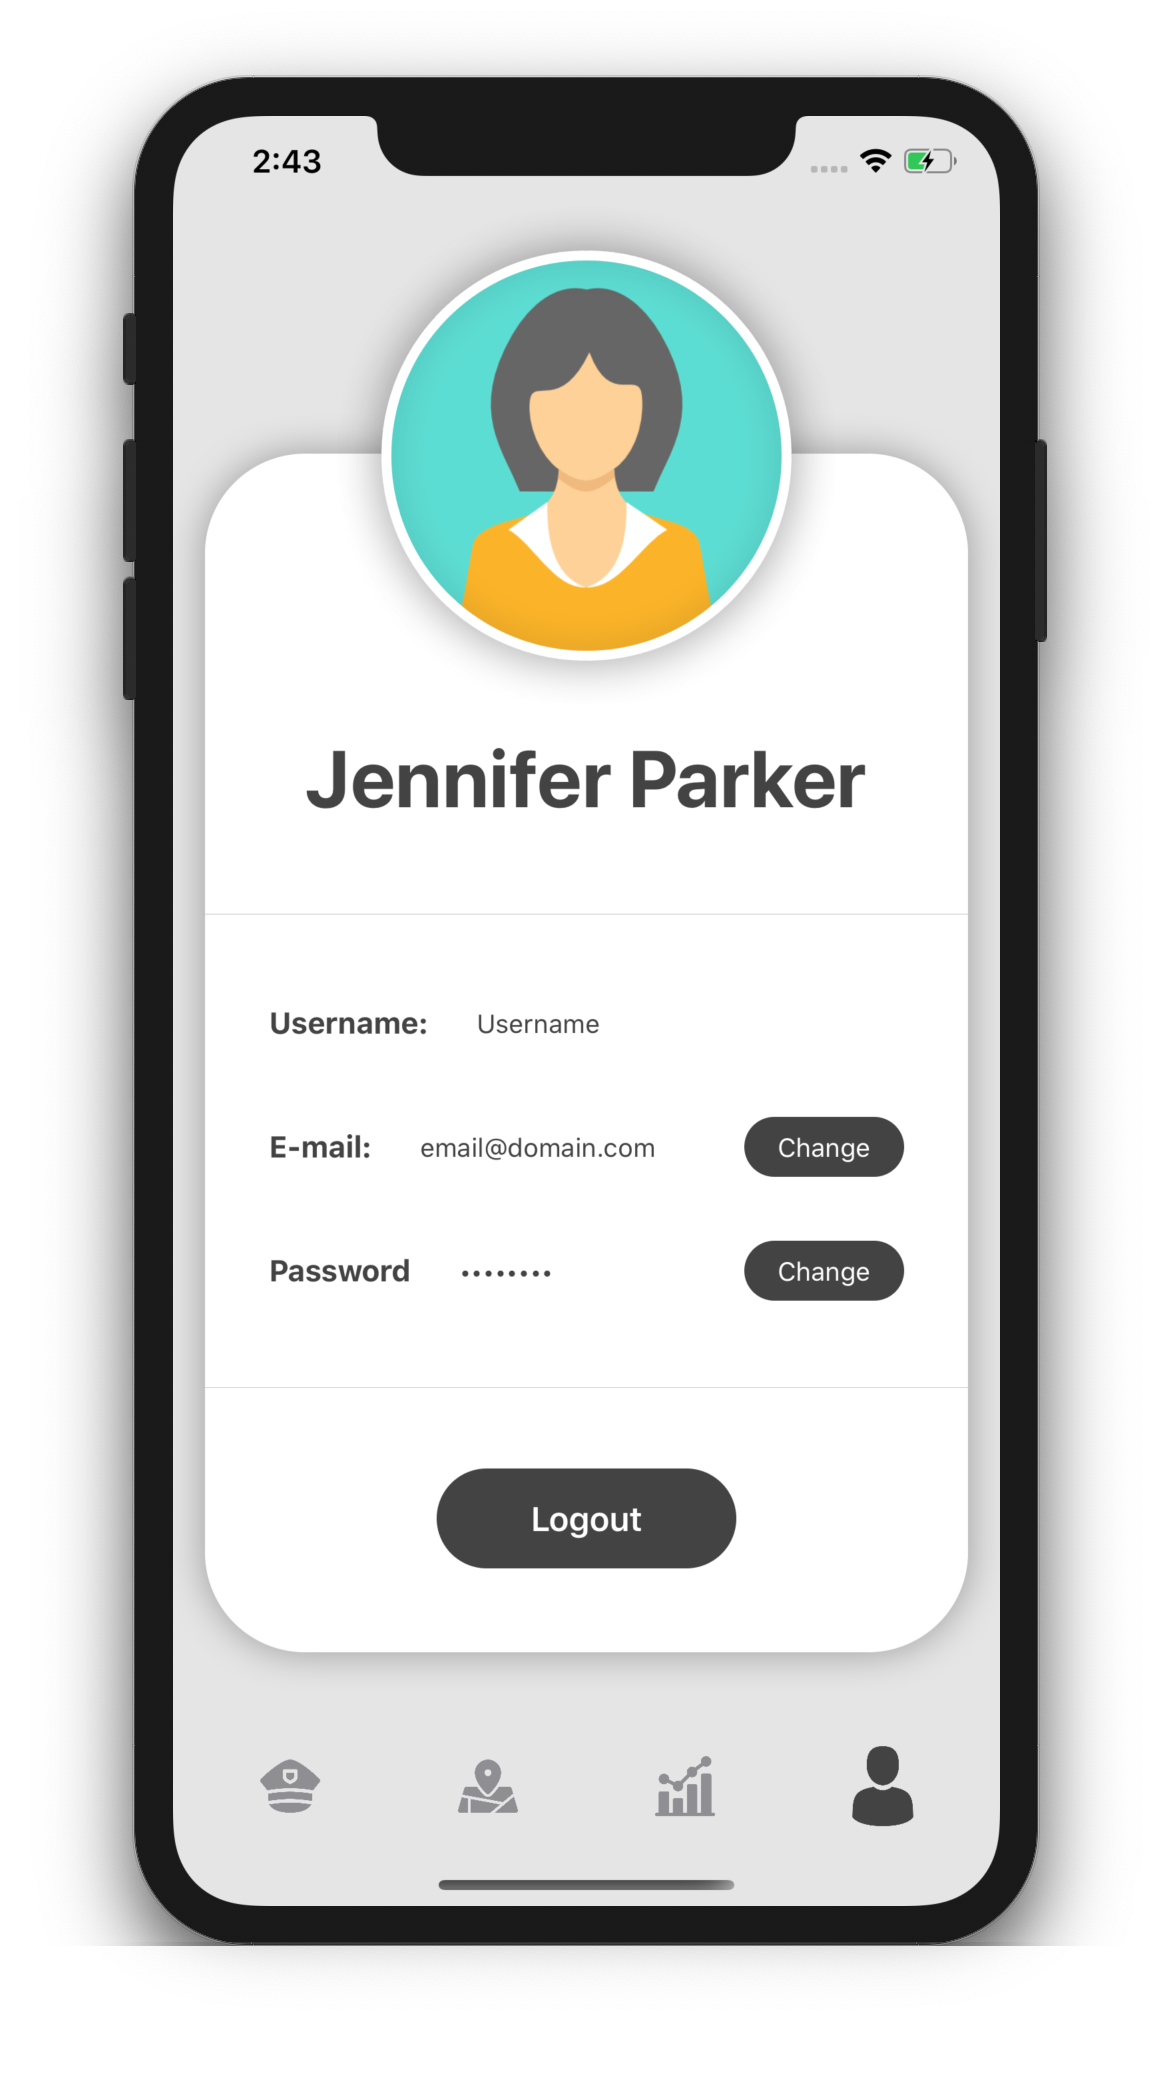
\includegraphics[width=\textwidth]{mockups/profile.png}
    				\caption{User Profile}
  				\end{minipage}
			\end{figure}
			
			\begin{figure}[h]
  				\centering
  				\begin{minipage}[b]{0.4\textwidth}
    				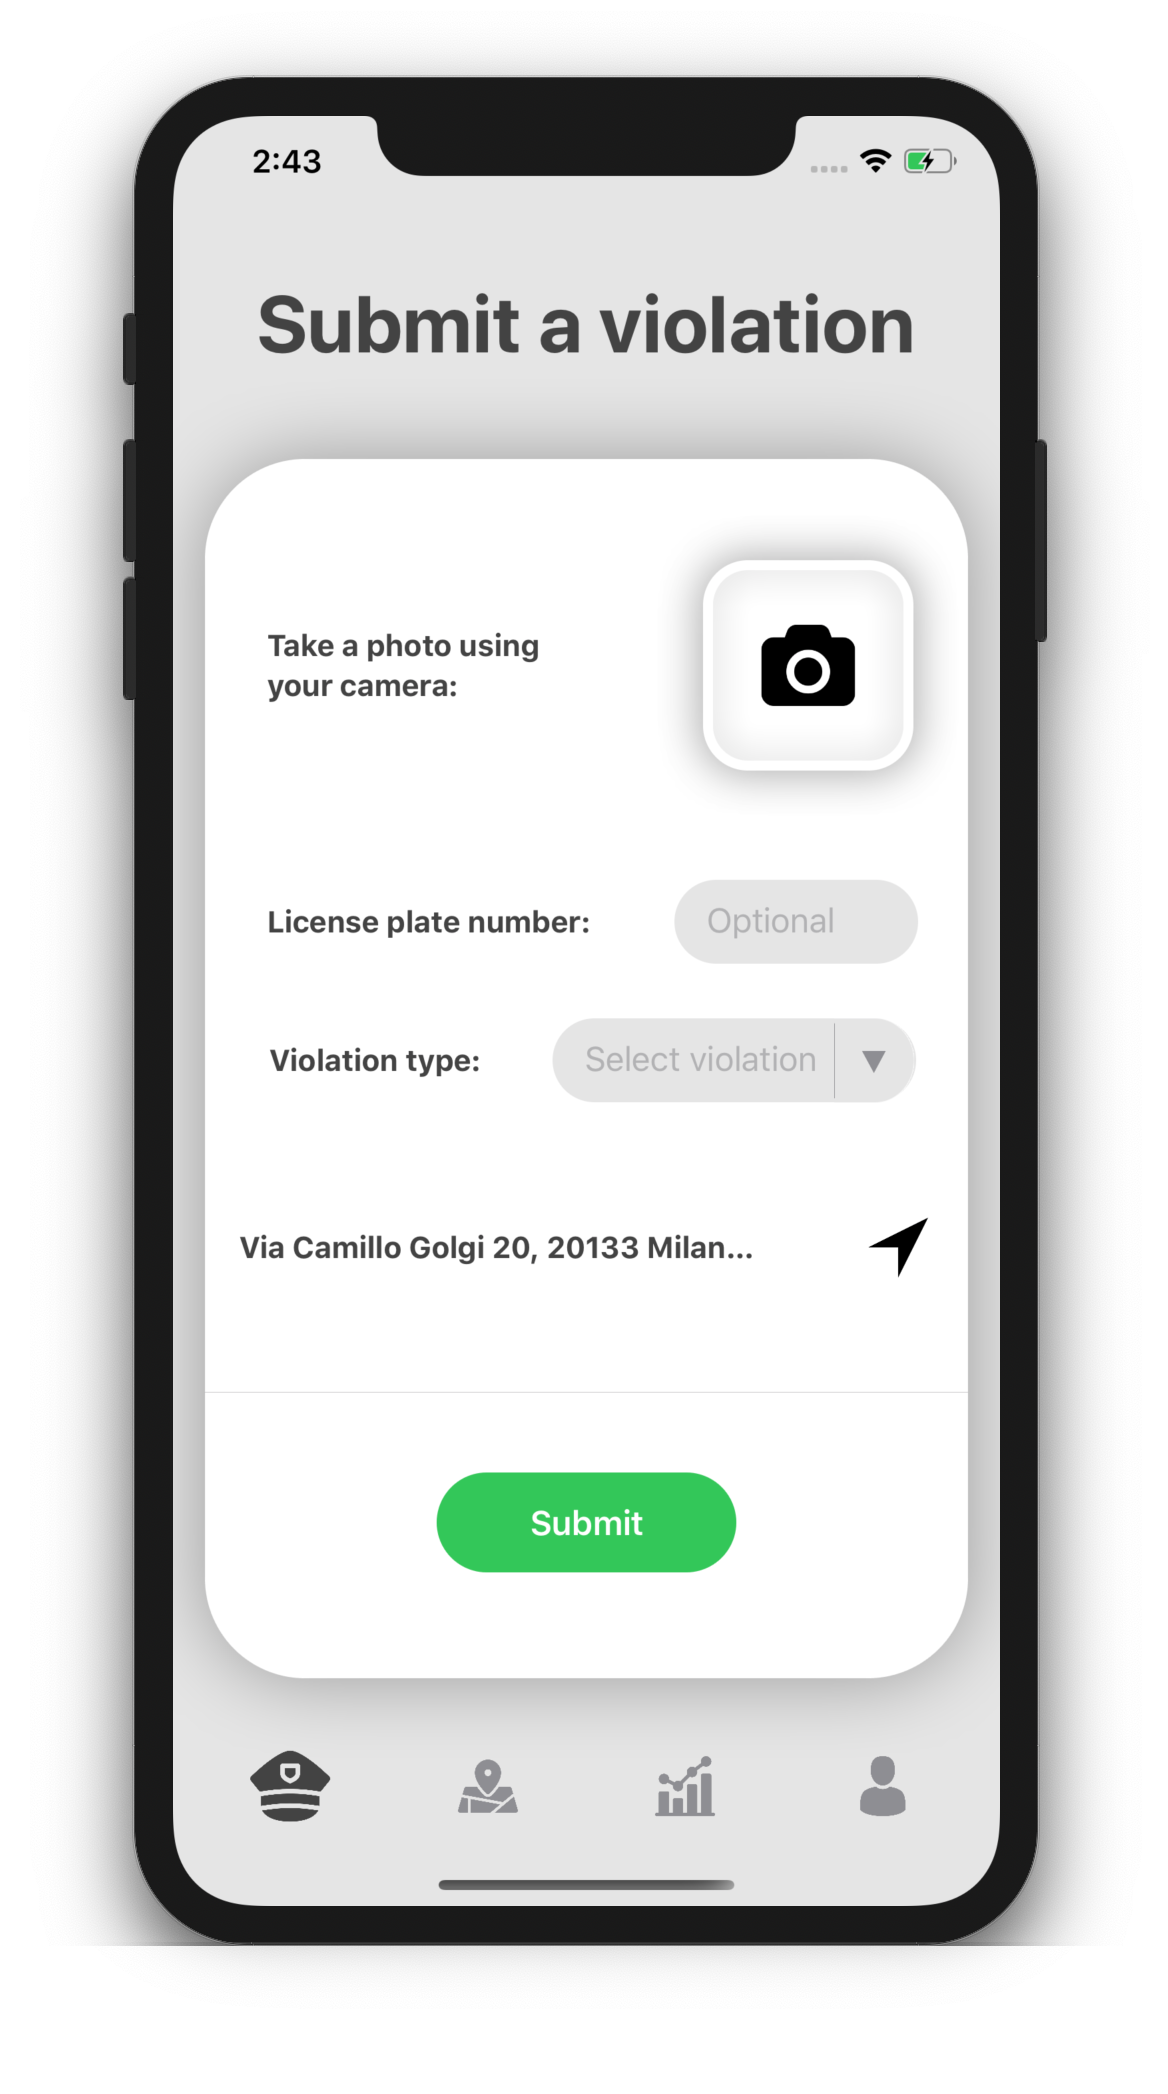
\includegraphics[width=\textwidth]{mockups/submit-violation.png}
    					\caption{Upload Procedure}
  				\end{minipage}
  				\hfill
  				\begin{minipage}[b]{0.4\textwidth}
    				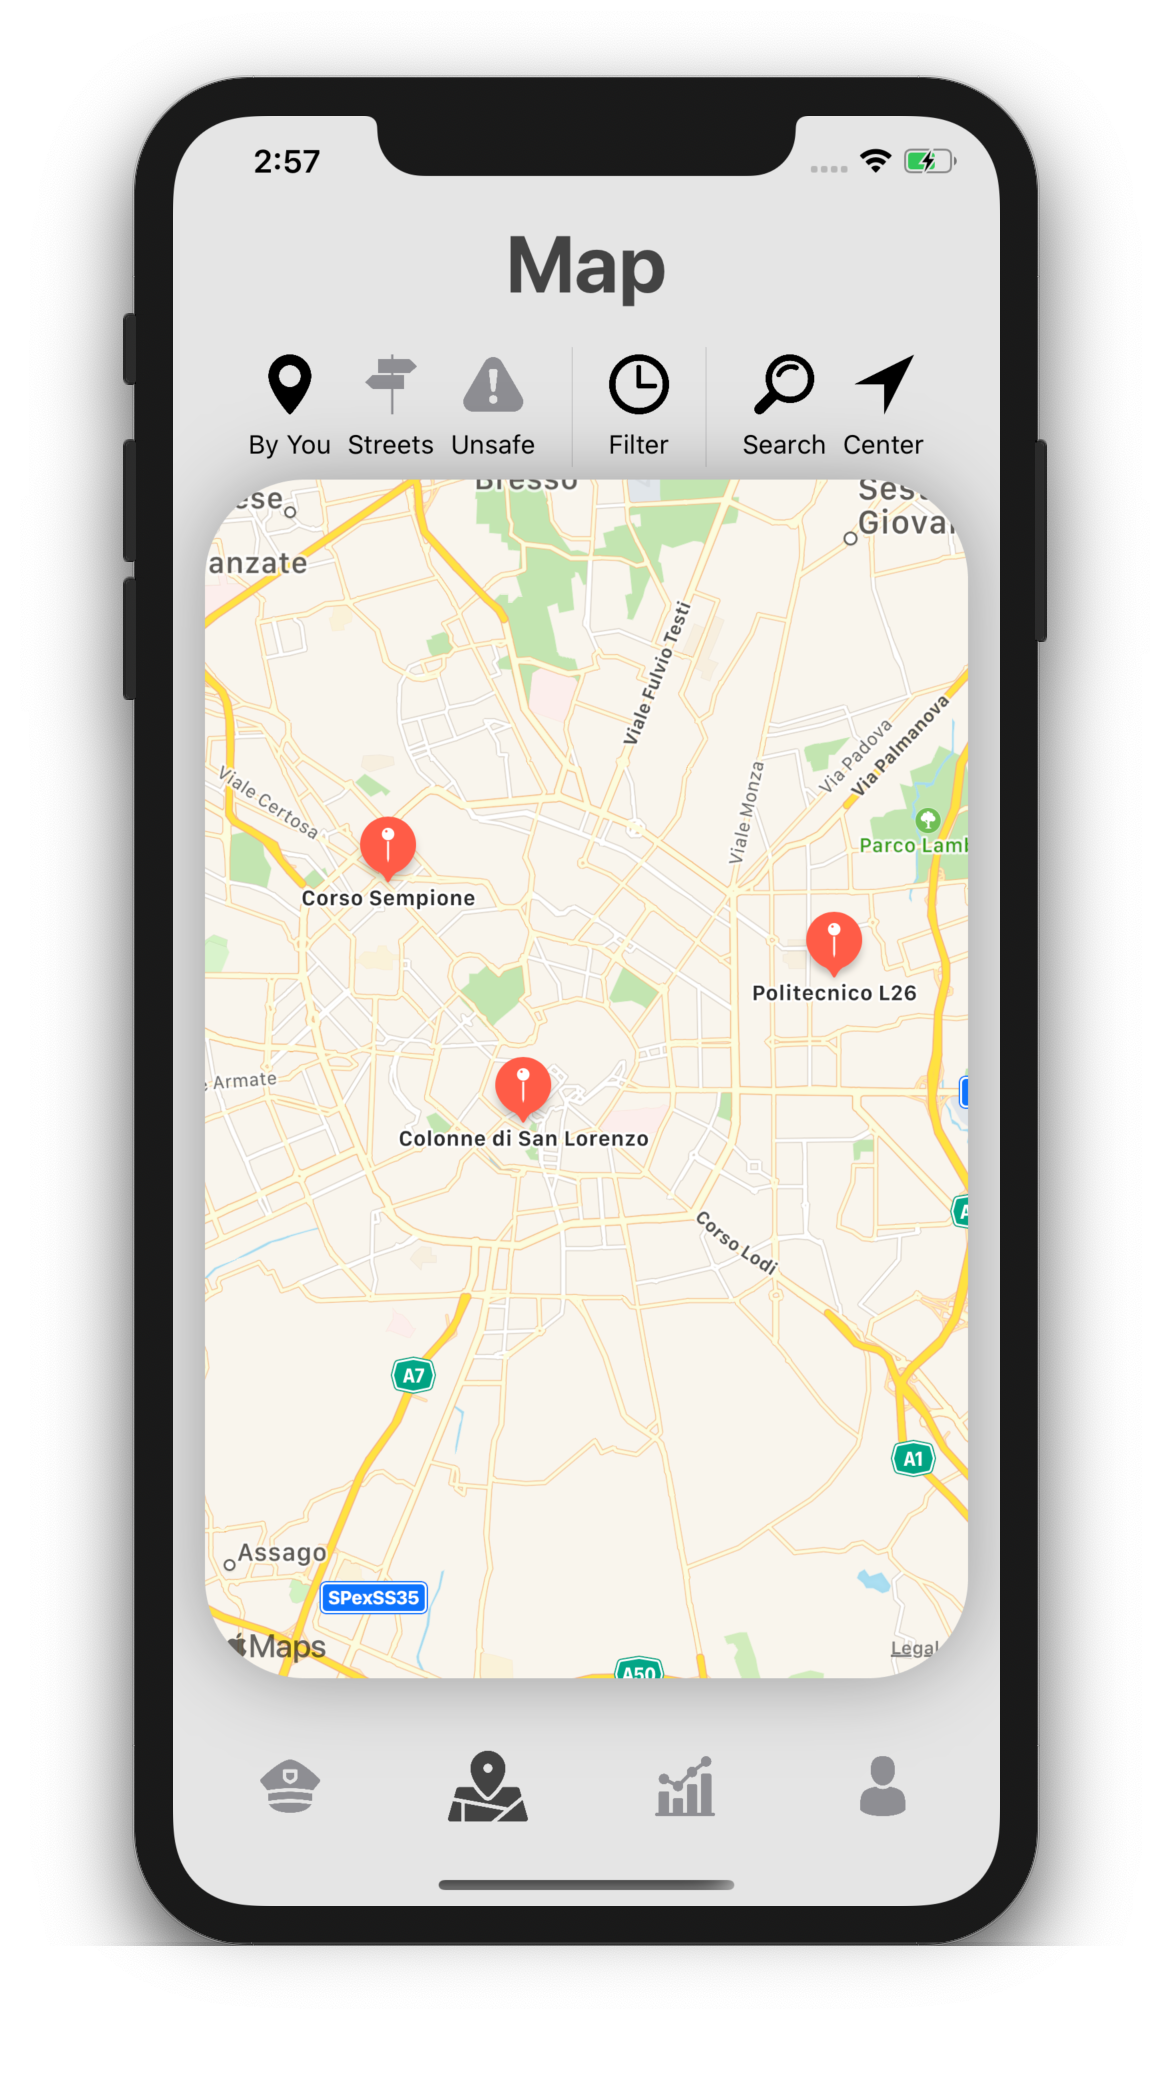
\includegraphics[width=\textwidth]{mockups/map.png}
    				\caption{Map Interface}
  				\end{minipage}
			\end{figure}
	\end{itemize}

\clearpage

\subsubsection{Hardware Interfaces}
	
\subsubsection{Software Interfaces}
\subsubsection{Communication Interfaces}

\clearpage

\subsection{Functional Requirements}

\subsubsection{Scenarios}

Application specific scenarios are presented to enrich the system's specification. These scenarios describe the usage of the system.

\paragraph{Scenario 1}
\label{scenario:1}
	Davide is walking down the street and notices a car parked over the crosswalks. He opens the SafeStreets app, registers to the system with his fiscal code, and takes a picture from the in-app camera. Before uploading he adds information such as the type of violation (i.e. "Bad Parking") and the street in which the violation occurred. As soon as SafeStreet processes the uploaded data the authorities are alerted.

\paragraph{Scenario 2}
\label{scenario:2}
	Carlo wants to teach his son to drive and wants to find the safest area of Milan in order to avoid exposing him to difficult situations in his first drives. He opens the SafeStreets app and consult the map with the streets that have the greatest number of incidents and violations, and will try to avoid them allowing his son to have a safe drive.

\paragraph{Scenario 3}
\label{scenario:3}
	SafeStreets automatically retrieves data from the municipality's service, and after a while notices that extremely frequently cars are parked in a prohibited restricted area of Milan. After further analysis and with the help of the users the system comes to the conclusion that drivers don't realise that they can't park in that area because of a misleading signal. SafeStreets  contacts the municipality and suggests a possible solution to the problem.

\paragraph{Scenario 4}
\label{scenario:4}
	After receiving a notification of "Dangerously parked car" with the picture showing a car parked in such a way that could risk a possible collision with the tram line, SafeStreets alerts the authorities in order to facilitate the process of car removal and the consequential ticket generation.
	
\clearpage

\subsubsection{Use Cases}

\clearpage

\subsubsection{Requirements Mapping}

	The following requirements are derived in order to achieve the specified goals.
	\begin{description}
		\item \ref{goal:register}\ Allow guest users to register to the system
			\begin{enumerate}[label=\textbf{R\arabic*}]
			
  				\item The system must require the \emph{guest} user to insert his fiscal code, a username, a valid e-mail and a password to identify him
  				
   				\item The system must check that the validity of the data inserted by the \emph{guest} user namely avoid duplicates, invalid fiscal codes and too weak passwords
   				
   				\item The system must send an e-mail to the \emph{guest} user to verify the e-mail address given during the registration
   
  			\end{enumerate}
  				
				\textbf{DA2} Internet connection always works correctly
				
				\textbf{DA6} The smartphone of the user runs iOS (9 or later) or Android (Jelly Bean or later)
			
  			
		\item \ref{goal:login}\ Allow registered users to authenticate to the system
			\begin{enumerate}[label=\textbf{R\arabic*}, resume]
  				\item The system must require the user to insert his username and password to authenticate to the system
   				\item The system must be able to check if the username and password pair correspond to a user correctly registered to the system and grant the access to that user

			\end{enumerate}
			
			\textbf{DA2} Internet connection always works correctly
			
			\textbf{DA5} The DBMS always works properly so that the information in the DB are always accessible
			
		\item \ref{goal:userTransfer}\ Allow users to transfer data to the system describing occurred violations, including the suitable metadata to describe the submitted violation			\begin{enumerate}[resume*]
				\item The system must allow the user to take a picture of the violation and the plate from the mobile application
  				\item The system must allow the user to manually insert the license plate number in order to help the recognition algorithm
  				\item The system must be able to retrieve the license plate of the vehicle running an algorithm to recognise it
  				\item The system must be able to verify that the license plate number is valid and registered to a vehicle
  				\item The system must require the user to specify the type of violation
  				\item The system must allow the user to provide the location of the violation, manually specifying the address, picking it up from the map or using the GPS of the device
   			\end{enumerate}
   			
   			\textbf{C2} The quality of the picture is sufficient to recognise the plate number (min resolution 320x240)
   			
			\textbf{C3} Internet connection must be strong enough to allow the upload of the picture in a reasonable amount of time (supported technologies are 3G, 4G and 5G due to the performance requirement)
			
			\textbf{DA1} GPS position of all users is always obtainable
			
			\textbf{DA2} Internet connection always works correctly
			
		\item \ref{goal:avoidLeaks}\ Ensure that the chain of custody of the information provided by the users is never broken, and the information is never altered or manipulated			\begin{enumerate}[resume*]
   				\item The system must provide a secure channel to communicate with the users
   				\item The system must encrypt the connection with the users in order to protect the process of providing data
   				\item The system must adopt security measures to prevent malicious accesses and to protect sensible data
   				\item Questo davvero non lo so mori miei
  			\end{enumerate}
  			
  			
		
		\item \ref{goal:municipalityTransfer}\ Allow the system to retrieve data about the accidents that occur on the territory and data about issued tickets via the municipality provided service
			\begin{enumerate}[resume*]
   				\item The system must be able to retrieve data about accidents from municipality systems 
   				\item The system must be able to process data retrieved from municipality
   				\item The system must be able to elaborate accidents and violations information to extract data about unsafe areas
   				\item The system must be able to provide data to municipality systems to suggest possible interventions to increase safety in a specific area
  			\end{enumerate}
  			
  			\textbf{DA2} Internet connection always works correctly
  			
			\textbf{DA3} Municipality services are always reachable
  			
  		\item \ref{goal:statistics}\ Allow the system to cross the information submitted by the users and the information retrieved from the municipality to build statistics
  			\begin{enumerate}[resume*]
  				\item 
   				
  			\end{enumerate}
  		\item \ref{goal:consultMap}\ Allow users to consult a map highlighting the streets (and the areas) with the highest frequency of violations, the identified potentially unsafe areas and view statistics about previously stored violations
  			\begin{enumerate}[resume*] 
  				\item The system must be able to retrieve data about tickets issued by the municipality 
   				\item The system must be able to process data retrieved from municipality
   				\item The system must be able to elaborate issued tickets information to generate statistics about useful violations provided by users
   			\end{enumerate}
   			
   			\item \ref{goal:retrieveData} Allow municipality to consult the system data and receive suggestions on possible interventions via a restrict access API 
   				\begin{enumerate}[resume*] 
  				\item The system must be able to retrieve data about tickets issued by the municipality 
   				\item The system must be able to process data retrieved from municipality
   				\item The system must be able to elaborate issued tickets information to generate statistics about useful violations provided by users
   			\end{enumerate}
   			
   	\end{description}

\subsection{Performance Requirements}

\subsection{Logical Database Requirements}

\subsection{Design Constraints}

\subsubsection{Standards Compliance}
\subsubsection{Hardware Limitations}
\subsubsection{Other?}

\subsection{Software System Attributes}

\subsubsection{Reliability}
\subsubsection{Availability}
\subsubsection{Security}
\subsubsection{Maintainability}
\subsubsection{Portability}

\clearpage

\section{Formal Analysis using Alloy}

\subsection{Source code}
		\lstinputlisting[language=alloy]{alloy/SafeStreets.als}
		
\subsection{Generated Worlds}

\clearpage





\subsection{Functional Requirements}


  	
\subsection{Performance Requirements}
	The system should ensure acceptable response times in the interactions with the user, which strictly depends on the number of concurrent users and the connection speed.
\newline
The processes of providing data and loading the map of safe and unsafe areas shouldn't be too slow.
\subsection{Software System Attributes}
	\subsubsection{Availability}
	The system must be available 99,9\% of the time (up to 8,76 hours per year of downtime). The system should be accessible 24 hours per day.
	\subsubsection{Security}
	Users personal information and payment information are encrypted and must be protected during transmission, as already stated the PTPP protocol will be used to ensure encryption through the network.
	Restricted access APIs must check that who tries to use them is actually allowed to do so.
	\subsubsection{Portability}
	The system must be also accessible by the most common mobile platforms (iOS and Android devices).

